%% 
%% Copyright 2007-2020 Elsevier Ltd
%% 
%% This file is part of the 'Elsarticle Bundle'.
%% ---------------------------------------------
%% 
%% It may be distributed under the conditions of the LaTeX Project Public
%% License, either version 1.2 of this license or (at your option) any
%% later version.  The latest version of this license is in
%%    http://www.latex-project.org/lppl.txt
%% and version 1.2 or later is part of all distributions of LaTeX
%% version 1999/12/01 or later.
%% 
%% The list of all files belonging to the 'Elsarticle Bundle' is
%% given in the file `manifest.txt'.
%% 

%% Template article for Elsevier's document class `elsarticle'
%% with numbered style bibliographic references
%% SP 2008/03/01
%%
%% 
%%
%% $Id: elsarticle-template-num.tex 190 2020-11-23 11:12:32Z rishi $
%%
%%
\documentclass[preprint,12pt]{elsarticle}

%% Use the option review to obtain double line spacing
%% \documentclass[authoryear,preprint,review,12pt]{elsarticle}

%% Use the options 1p,twocolumn; 3p; 3p,twocolumn; 5p; or 5p,twocolumn
%% for a journal layout:
%% \documentclass[final,1p,times]{elsarticle}
%% \documentclass[final,1p,times,twocolumn]{elsarticle}
%% \documentclass[final,3p,times]{elsarticle}
%% \documentclass[final,3p,times,twocolumn]{elsarticle}
%% \documentclass[final,5p,times]{elsarticle}
%% \documentclass[final,5p,times,twocolumn]{elsarticle}

%% For including figures, graphicx.sty has been loaded in
%% elsarticle.cls. If you prefer to use the old commands
%% please give \usepackage{epsfig}

%% The amssymb package provides various useful mathematical symbols
\usepackage{amssymb}
\usepackage{longtable}
\usepackage{array}

%% The amsthm package provides extended theorem environments
%% \usepackage{amsthm}

%% The lineno packages adds line numbers. Start line numbering with
%% \begin{linenumbers}, end it with \end{linenumbers}. Or switch it on
%% for the whole article with \linenumbers.
%% \usepackage{lineno}

\journal{Nuclear Physics B}

\begin{document}

\begin{frontmatter}

%% Title, authors and addresses

%% use the tnoteref command within \title for footnotes;
%% use the tnotetext command for theassociated footnote;
%% use the fnref command within \author or \address for footnotes;
%% use the fntext command for theassociated footnote;
%% use the corref command within \author for corresponding author footnotes;
%% use the cortext command for theassociated footnote;
%% use the ead command for the email address,
%% and the form \ead[url] for the home page:
%% \title{Title\tnoteref{label1}}
%% \tnotetext[label1]{}
%% \author{Name\corref{cor1}\fnref{label2}}
%% \ead{email address}
%% \ead[url]{home page}
%% \fntext[label2]{}
%% \cortext[cor1]{}
%% \affiliation{organization={},
%%             addressline={},
%%             city={},
%%             postcode={},
%%             state={},
%%             country={}}
%% \fntext[label3]{}

\title{Terramycelium: A Complex Adaptive Reference Architecture for Big Data Sytems}

%% use optional labels to link authors explicitly to addresses:
%% \author[label1,label2]{}
%% \affiliation[label1]{organization={},
%%             addressline={},
%%             city={},
%%             postcode={},
%%             state={},
%%             country={}}
%%
%% \affiliation[label2]{organization={},
%%             addressline={},
%%             city={},
%%             postcode={},
%%             state={},
%%             country={}}

\author[inst1]{Author One}

\affiliation[inst1]{organization={Department One},%Department and Organization
            addressline={Address One}, 
            city={City One},
            postcode={00000}, 
            state={State One},
            country={Country One}}

\author[inst2]{Author Two}
\author[inst1,inst2]{Author Three}

\affiliation[inst2]{organization={Department Two},%Department and Organization
            addressline={Address Two}, 
            city={City Two},
            postcode={22222}, 
            state={State Two},
            country={Country Two}}

\begin{abstract}
%% Text of abstract
Lorem ipsum dolor sit amet, consectetur adipiscing elit, sed do eiusmod tempor incididunt ut labore et dolore magna aliqua. Ut enim ad minim veniam, quis nostrud exercitation ullamco laboris nisi ut aliquip ex ea commodo consequat. Duis aute irure dolor in reprehenderit in voluptate velit esse cillum dolore eu fugiat nulla pariatur. Excepteur sint occaecat cupidatat non proident, sunt in culpa qui officia deserunt mollit anim id est laborum.
\end{abstract}

%%Graphical abstract
% \begin{graphicalabstract}
% \includegraphics{grabs}
% \end{graphicalabstract}

%%Research highlights
\begin{highlights}
\item Research highlight 1
\item Research highlight 2
\end{highlights}

\begin{keyword}
%% keywords here, in the form: keyword \sep keyword
keyword one \sep keyword two
%% PACS codes here, in the form: \PACS code \sep code
\PACS 0000 \sep 1111
%% MSC codes here, in the form: \MSC code \sep code
%% or \MSC[2008] code \sep code (2000 is the default)
\MSC 0000 \sep 1111
\end{keyword}

\end{frontmatter}


\section{Introduction}
\label{sec:introduction}

The advent of the internet and widespread use of digital devices have sparked a profound shift in connectivity and data creation, leading to an era marked by a rapid growth in data. This period is characterised by the extensive expansion of data, which presents difficulties for traditional data processing systems and necessitates inventive methods in data architecture \cite{AtaeiACIS,AtaeiBigDataEnvirons}. The vast amount, variety, and rapid generation of data in the current digital environment necessitate innovative solutions, particularly in the field of Big Data (BD).

Data needs have dramatically evolved, transitioning from basic business intelligence (BI) functions, like generating reports for risk management and compliance, to incorporating machine learning across various organisational facets \cite{ataei2023towards}. These range from product design with automated assistants to personalised customer service and optimised operations.  Also, as machine learning becomes more popular, application development needs to change from rule-based, deterministic models to more flexible, probabilistic models that can handle a wider range of outcomes and need to be improved all the time with access to the newest data. This evolution underscores the need to reevaluate and simplify our data management strategies to address the growing and diverse expectations placed on data.

Currently, the success rate of BD projects is low. Recent surveys have identified the fact that current approaches to big data do not seem to be effectively addressing these expectations. According to a survey conducted by \cite{DataBricksSurvey}, only 13\% of organisations are highly successful in their data strategy. Additionally, a report by NewVantage Partners reveals that only 24\% of organisations have successfully converted to being data-driven, and a measly 30\% have a well-established big data strategy. These observations, additionally corroborated by research conducted by McKinsey \& Company (analytics2016age) and Gartner (Nash), emphasise the difficulties of successfully using big data in the industry. These difficulties include the lack of a clear understanding of how to extract value from data, the challenge of integrating data from multiple sources, data architecture, and the need for skilled data analysts and scientists. 

Without a well-established big data strategy, companies may struggle to navigate these challenges and fully leverage the potential of their data. One effective artefact to overcome some of these challenges is Reference Architectures (RAs) \cite{Cloutier2010}. RAs extract the essence of the practice as a series of patterns and architectural constructs and manifest it through high-level semantics. This allows stakeholders to refrain from reinventing the wheel and instead focus on utilising existing knowledge and best practices to harness the full potential of their data. While there are various BD RAs available to help practitioners design their BD systems, these RAs are overly cetnralised, lack attention to cross-cutting concerns such as privacy, security, and metadata, and may not effectively handle the proliferation of data sources and consumers.

To this end, this study presents TerrMycelium, a distributed RA designed specifically for BD systems with a focus on domain-driven design. TerrMycelium seeks to surpass the constraints of current RAs by utilising domain-driven and distributed approaches derived from contemporary software engineering. This method aims to improve the ability of BD systems to scale, be maintained, and evolve, surpassing the constraints of traditional monolithic data architectures.

The paper is structured as follows: Section~\ref{sec:background} provides an overview of the foundational concepts and technologies pertinent to BD reference architecture, aiming to forge a conceptual framework that is required for this paper. An overview of the existing research on the topic is presented in Section~\ref{sec:related_work}. The significance of reference architectures in the context of big data is explored in Section~\ref{sec:why_reference_architectures}. Section~\ref{sec:software_and_system_requirements} details the software and system requirements necessary for implementing the proposed architecture. Section~\ref{sec:theory} delves into the theoretical foundation underpinning the challenges in contemporary big data systems. The design and development of the TerrMycelium artifact are described in Section~\ref{sec:artifact}. Section~\ref{sec:discussion} examines the evaluation findings, their implications, limitations, and relevance to existing and future research. Finally, Section~\ref{sec:conclusion} summarizes the main contributions of the study, its practical implications, and suggests directions for future research.


\section{Background}
\label{sec:background}

This section provides foundational definitions essential for comprehending the nuances of the research. This chapter aims to create the conceptual framework necessary to understand the terminology used in the thesis.

\subsection{What is Big Data?}

To define BD within the scope of this research, various academic definitions have been examined. \citet{Kaisler2013} define BD as ``the amount of data which is beyond technology’s capability to store, manage and process efficiently''.
\citet{Srivastava2018} state that BD pertains to ``the use of large data sets to handle the collection or reporting of data that serves various recipients in decision making''.

\citet{Sagiroglu2013} describe BD as ``a term for massive data sets having large, more varied and complex structure with the difficulties of storing, analyzing and visualizing for further processes or results''. 

Drawing from these definitions, BD in this research is conceptualised as the endeavour to discern patterns from vast amounts of data for the objectives of advancement, governance, and predictive analysis in domain-specific applications.

\subsection{The Value of Big Data}\label{sec:The Value of Big Data}

The significance and value derived from BD remain pronounced \cite{ataei2022state}. Extensive discussions on the concept permeate reports, statistics, researches, and conferences \cite{Chen2012}. Notably, prominent companies like Google, Facebook, Netflix, and Amazon have propelled this momentum with substantial investments in BD initiatives \cite{Rada2017}.

A compelling illustration of the tangible benefits that BD offers can be seen in the Netflix Prize recommender system. This system capitalized on a diverse array of data sources, including user queries, ratings, search terms, and various demographic indicators \cite{Amatriain2013}. By implementing BD-powered recommendation algorithms, Netflix not only achieved a considerable increase in TV series consumption but also observed certain series experiencing up to a fourfold surge in viewership \cite{Amatriain2013}.


In a healthcare context, the Taiwanese government adeptly merged its national health insurance database with customs and immigration datasets as part of a BD strategy \cite{wang2020response}. The resulting real-time alerts during clinical visits, informed by clinical symptoms and travel history among other factors, facilitated proactive identification of potential COVID-19 cases. Such strategic data-driven initiatives significantly bolstered Taiwan's effectiveness in managing the epidemic.

In the realm of energy exploration, Shell harnesses BD to optimise the decision-making process and reduce exploration costs \cite{Marr2016}. By uploading and comparing data from various drilling sites globally, decisions pivot towards locations that mirror those with confirmed abundant resources. Prior to BD's integration, identifying energy resources presented formidable challenges. Traditional exploration methods, which relied heavily on deciphering waves of energy travelling through the earth's crust, were not only error-prone but also exorbitantly expensive and time-intensive.

Similarly, Rolls Royce capitalises on BD's potential by collecting intricate performance data from sensors fitted on its aircraft products \cite{Marr2016}. Such data, transmitted wirelessly, provides insights into key operational phases, from take-off to maintenance. Leveraging this wealth of information, Rolls Royce can more accurately detect degradation, enhance diagnostic and prognostic accuracy, and effectively reduce false positives.

\subsection{Reference Architectures}

RAs have emerged as pivotal elements in contemporary system development, guiding the construction, maintenance, and evolution of increasingly complex systems \cite{Cloutier2010}. They offer a clear depiction of the essential components of a system and the interactions necessary to realize overarching objectives. This clarity fosters the creation of manageable modules, each addressing distinct aspects of complex problems, and provides a high-level platform for stakeholders to engage, contribute, and collaborate.

The significance of RAs in IT is underscored by the success of widely adopted technologies like OAuth \cite{OATH} and ANSI-SPARC architecture \cite{ANSI}, which have their origins in well-structured RAs. These RAs not only define the qualities of a system but also shape its evolution. While every system inherently possesses an architecture, RAs distinguish themselves by focusing on more abstract qualities and higher levels of abstraction. They aim to capture the essence of practice and integrate well-established patterns into cohesive frameworks, encompassing elements, properties, and interrelationships.

The significance of RAs in BD is multifaceted, encompassing aspects like communication, complexity control, knowledge management, risk mitigation, fostering future architectural visions, defining common ground, enhancing understanding of BD systems, and facilitating further analysis.

\subsection{Microservices and Decentralised, Distributed Architectures}

Microservices architecture, representing an evolution in software engineering, involves structuring applications as a collection of loosely coupled services \cite{bucchiarone2020microservices}. This approach, emerging from the broader concept of Service Oriented Architectures (SOA), focuses on developing small, independently deployable modules that collaborate to form a comprehensive application. As \citet{Newman2015} elucidates, microservices enhance scalability, facilitate continuous deployment, and foster a more agile development environment. They enable teams to develop, deploy, and scale parts of a system independently, thus improving overall system resilience and facilitating rapid adaptation to changing demands.

Decentralised and distributed architectures are integral to the modern computing landscape, characterised by systems spread across multiple nodes, often in different geographic locations. This architectural style, as highlighted by \citet{Richards2015}, mitigates the limitations of traditional monolithic structures, offering enhanced scalability, fault tolerance, and flexibility. In distributed systems, data and processing are dispersed across multiple nodes, which interact with each other to perform tasks, as discussed by \citet{Coulouris2005}. Decentralisation in this context implies the lack of a single controlling node, instead opting for a more democratic and resilient network structure.

The convergence of microservices within these architectures represents a progressive step in software engineering. It reflects a move towards systems that are not only distributed in nature but also modular and adaptable. This architectural approach aligns well with contemporary demands for systems that are scalable, resilient, and capable of leveraging the distributed nature of modern computing environments. The adoption of microservices in decentralised, distributed architectures heralds a new era in software development, where flexibility, scalability, and resilience are paramount.




\section{Related Work}
\label{sec:related_work}

This section reviews seminal works in BD RAs, delineating their scope, methodologies, and inherent limitations, thereby justifying the novel approach of this study's domain-driven distributed RA, \textit{Terramycelium}.

Lambda architecture \cite{kiran2015lambda} and Kappa architecture \cite{kreps2014questioning} represent pivotal industry contributions to BD RAs, introducing foundational paradigms for data processing. However, these architectures have faced criticism for their lack of comprehensive data management strategies, particularly regarding data quality, security, and metadata \cite{AtaeiACIS}. This gap is further evidenced in domain-specific RAs like those proposed by \cite{quintero2019ibm} for healthcare, which, while addressing domain-specific needs, often overlook cross-cutting concerns such as privacy and interoperability.

Academic efforts, as in \cite{viana2014proposal} and \cite{paakkonen2015reference}, have aimed to broaden the conceptual understanding of BD systems, proposing RAs that attempt to encapsulate more holistic views of data analytics ecosystems. Yet, these proposals frequently fall short in addressing the dynamic and distributed nature of modern data landscapes, particularly in terms of scalability and modifiability.

The limitations of current BD RAs, as summarized in the works of \citeauthor{ataei2022state}, highlight a common trend: a pronounced reliance on monolithic data pipeline architectures. This reliance is manifest in the inadequacy of existing RAs to effectively manage data quality, security, privacy, and metadata. Furthermore, the monolithic nature of these architectures often results in scalability and modifiability issues, as they struggle to adapt to the evolving data and technology landscapes.

Against this backdrop, \textit{Terramycelium} emerges as a novel RA for BD systems. By embracing a domain-driven, distributed approach, \textit{Terramycelium} addresses the critical limitations identified in existing RAs. Unlike its predecessors, which often encapsulate data management within rigid, monolithic structures, \textit{Terramycelium} advocates for decentralized data stewardship and a modular architecture. This approach not only enhances scalability and flexibility but also ensures that cross-cutting concerns such as security, privacy, and data quality are inherently integrated into the system's design.

In essence, \textit{Terramycelium} represents a significant departure from traditional BD RAs. By prioritizing domain-driven design and distributed processing, it offers a scalable and adaptable framework that aligns more closely with contemporary data management needs and the principles of modern software architecture. In doing so, \textit{Terramycelium} not only addresses the limitations of existing RAs but also positions itself as a vanguard in the evolution of BD system design, paving the way for future research and development in this critical field.

\section{Why Reference Architectures}
\label{sec:why_reference_architectures}

Conceptualisation of the system as an RA, helps with understanding of the system’s key components, behaviour, composition and evolution of it, which in turn affect quality attributes such as maintainability, scalability and performance \cite{Cloutier}. 

Therefore, RAs can be a good standardisation artefact and a communication medium that not only results in concrete architectures for BD systems, but also provide stakeholders with unified elements and symbols to discuss and progress BD projects.

The practice of leveraging RAs for both system conceptualisation and as a standardisation artefact is not new to practitioners of complex systems. In Software Product Line (SPL) development, RAs are utilised as generic artifacts that are instantiated and configured for a particular domain of systems \cite{Derras}. 

In software engineering, renowned IT corporations such as IBM have consistently advocated for RAs, considering them exemplary practices in addressing intricate system design challenges \cite{Cloutier2010}. Similarly, in the realm of international standards, RAs frequently serve as tools to standardize emerging domains. 

Morover, the BS ISO/IEC 18384-1 RA for service-oriented architectures \cite{Iso18384-1} demonstrates the utility of RAs in creating standardized frameworks in specific fields.

\section{Software and System Requirements}
\label{sec:software_and_system_requirements}

According to \citeauthor{wieringa2014design}\cite{wieringa2014design}, the requirement specification phase is an essential step in developing a new IS or artefact. This phase involves identifying the requirements that the artefact must satisfy to meet the needs of stakeholders and achieve the desired outcomes.

\citeauthor{wieringa2014design}'s methodology distinguishes between functional requirements, which describe what the artefact should do, and non-functional requirements, which describe how the artefact should do it. Functional requirements are typically expressed as use cases, which describe the specific interactions between users and the system. Non-functional requirements may include performance requirements, security requirements, and usability requirements.

The requirement specification designed for this study is made up of the following phases: 

\begin{enumerate}
    \item Determining the type of the requirements 
    \item Determining the relevant requirements and 
    \item Identifying the right approach for categorisation of the requirements 
    \item Identifying the right approach for the presentation of the requirements 
\end{enumerate}

\paragraph{Determining the type of the requirements:}

Defining and classifying software and system requirements is a common subject of debate. \citeauthor{sommerville2011software}\cite{sommerville2011software} classify requirements as three levels of abstraction; user requirements, system requirements, and design specifications. These abstractions are then mapped against user acceptance testing, integration testing, and unit testing. Nevertheless, in this study, a more general framework provided by \citeauthor{laplante2017requirements} is adopted. The adopted approach provides three types of requirements: functional, non-functional, and domain requirements. The objective of this step is to define the high-level requirements of BD systems, therefore the main focus is on non-functional and domain requirements. 

\paragraph{Determining the relevant requirements:}

In an extensive effort, the NIST Big Data Public Working Group embarked on a large-scale study to extract requirements from a variety of application domains such as Healthcare, Life Sciences, Commercial, Energy, Government, and Defense \cite{Chang}. The result of this study is the formation of general requirements under seven categories. In addition, \citeauthor{volk2020identifying} categorize nine use cases of BD projects sourced from published literature using a hierarchical clustering algorithm. 

\citeauthor{AtaeiSecurity}\cite{AtaeiSecurity} focus on security and privacy requirements for BD systems, \citeauthor{yu2019components} present modern components of BD systems, using goal-oriented approaches, \citeauthor{eridaputra2014modeling} created a generic model for BD requirements, and  \citeauthor{al2016characteristics} investigate general requirements to support BD software development. 

By analyzing the result of the first SLRs, the studies discussed above and by evaluating the design and requirement engineering required for BD RAs, a set of high-level requirements based on BD characteristics is established. 

\paragraph{Identifying the right approach for categorisation of the requirements:}

After clarifying the type of requirements and the relevant requirements, current BD RAs and their requirements have been assessed to increase understanding of the available BD requirement categorisation methods. A common theme among these studies connected the dot towards a common approach to classifying requirements. This approach is categorised through BD characteristics such as velocity, veracity, volume, variety, value, security and privacy \cite{ataei2022state, Bahrami2015,rad2017big,Chen2016a}.

\paragraph{Identifying the right approach for the presentation of the requirements:}

Then, a rigorous approach to present software and system requirements that offers informal methods of model verification is identified because such methods are well established in the industry and academia \cite{kassab2014state}. The approach for representing functional requirements follows the guidelines in \emph{ISO/IEC/IEEE standard 29148} \cite{ISO29148}. 

The requirements representation is organized in system modes, where the major components of the system and then the requirements are described. This approach is inspired by the requirement specification expressed for NASA Wide-field InfraRed Explorer (WIRE) system \cite{laplante2017requirements} and the Software Engineering Body of Knowledge (SEBoK) \cite{abran2004software}. These requirements are described in Table~\ref{table:systemRequirements}.


\begin{longtable}{|m{1.4cm}|m{12cm}|}
  \caption{Terramycelium software and system requirements}
  \label{table:systemRequirements}\\
  \hline

          Volume &
  
          \textbf{Vol-1)}\label{vol-1} System needs to support asynchronous, streaming, and batch processing to collect data from centralised, distributed, and other sources
          
          \textbf{Vol-2)} System needs to provide scalable storage for massive data sets 
          \\
          \hline
          Velocity & 
          
          \textbf{Vel-1)} System needs to support slow, bursty, and high throughput data transmission between data sources
          
          \textbf{Vel-2)} System needs to stream data to data consumers in a timely manner
          
          \textbf{Vel-3)} System needs to be able to ingest multiple, continuous, time-varying data streams 
          
          \textbf{Vel-4)} System shall support fast search from streaming and processed data with high accuracy and relevancy 
          
          \textbf{Vel-5)} System should be able to process data in a real-time or near real-time manner 
          \\ 
  
          \hline
  
          Variety & 
  
          \textbf{Var-1)} System needs to support data in various formats ranging from structured to semi-structured and unstructured data 
          
          \textbf{Var-2)} System needs to support aggregation, standardization, and normalization of data from disparate sources
          
          \textbf{Var-3)} System shall support adaptations mechanisms for schema evolution
          
          \textbf{Var-4)} System can provide mechanisms to automatically include new data sources 
          \\
  
          \hline
  
          Value & 
          
          \textbf{Val-1)} System needs to able to handle compute-intensive analytical processing and machine learning techniques 
          
          \textbf{Val-2)} System needs to support two types of analytical processing: batch and streaming
          
          \textbf{Val-3)} System needs to support different output file formats for different purposes 
          
          \textbf{Val-4)} System needs to support streaming results to the consumers 
          \\
  
          \hline
  
          Security \& Privacy & 
          
          \textbf{SaP-1)} System needs to protect and retain the privacy and security of sensitive data 
          
          \textbf{SaP-2)} System needs to have access control, and multi-level, policy-driven authentication on protected data and processing nodes. 
          \\
  
          \hline
          
          Veracity &
          
          \textbf{Ver-1)} System needs to support data quality curation including classification, pre-processing, format, reduction, and  transformation 
          
          \textbf{Ver-2)} System needs to support data provenance including data life cycle management and long-term preservation.
          \\
          \hline
  
  \end{longtable}


\section{Theory}
\label{sec:theory}

In mathematical terms, an inflection point is a significant juncture where the curvature of a curve changes direction, signifying the transition from one behaviour to another. This pivotal point is marked by a dissolution of the prior shape and the emergence of a novel form. Today, there are empirical signals and derivers that point in the direction of a seismic shift \cite{mit_tech_review_2023}. 
s
A glimpse of the New Vantage Partners report in 2023 communicates that despite potential economic headwinds, the investments in data are growing and remain strong. Nevertheless, the report also communicates that only 23.9\% of companies identify themselves as data-driven. 

Before discussing these design theories, a clear communication method for architectural constructs is essential. This study employs the architecture definition from ISO/IEC 42010 \cite{ISO42010}, described as 'the fundamental concepts or properties of a system in its environment embodied in its elements, relationships, and in the principles of its design and evolution'.

\subsection{The monolith}

While the tools and technologies of data engineering have reached the Cambrian explosion \cite{AtaeiHype}, the underlying assumptions that govern the data architectures have not been much challenged.

According to \citeauthor{richards2020fundamentals} there are two major categories of architectures; 1) monolithic (deployed as a single unit) and 2) distributed (the system is made up of sub-components that are deployed separately). Today, most data architectures are in the first category. 

While starting as a monolith can be a simple and good approach for building a data-intensive system, it falls short as the solution scales. While this assumption is challenged in the software engineering world, data engineering seems to still be driven by monolithic designs \cite{ataei2022state}. These designs are enforced by enabler technologies such as data warehouses and data lakes. In addition, many organisations and books adopt the idea of a \emph{single source of truth}.

\subsection{The data chasm}

Analytical data and operational data are two distinct types of data used in businesses. Operational data is used to manage day-to-day business operations, while analytical data is used to support strategic decision-making by identifying patterns and trends in historical data.

Many of the challenges of current BD architectures rely on its fundamental assumption of dividing operational and analytical data. While operational and analytical data have different properties and are processed differently, bringing operational data far from its original source can affect its integrity negatively, create organisational silos, and produce data quality issues. 

These two different planes of data are usually operated underlying different organisational hierarchies. Data scientists, business intelligence analysts, machine learning engineers, data stewards, and data engineers are usually under the leadership of the Chief Data and Analytics Officer (CDAO) and are heavily involved in creating business value out of data. On the other hand, software engineers, product owners, and quality assurance engineers are usually working with the Chief Technology Officer (CTO).

This has resulted in two segregated technology stacks and heavy investments in bridging the two. This chasm has resulted in two different topologies and fragile integration architectures through ETLs (Figure \ref{fig:dataPlanes}). This is usually achieved by some sort of batch ETL job that aims to extract data from operational databases. These ETLs usually don't have any clearly defined contract with the operational database and are sheer consumers of its data. This highlights the fragility of this architecture, as the upstream changes from operational databases can affect downstream analytical applications. Over time, ETL job complexity increases, maintainability becomes harder, and data quality decreases. 

\begin{figure}[h]
  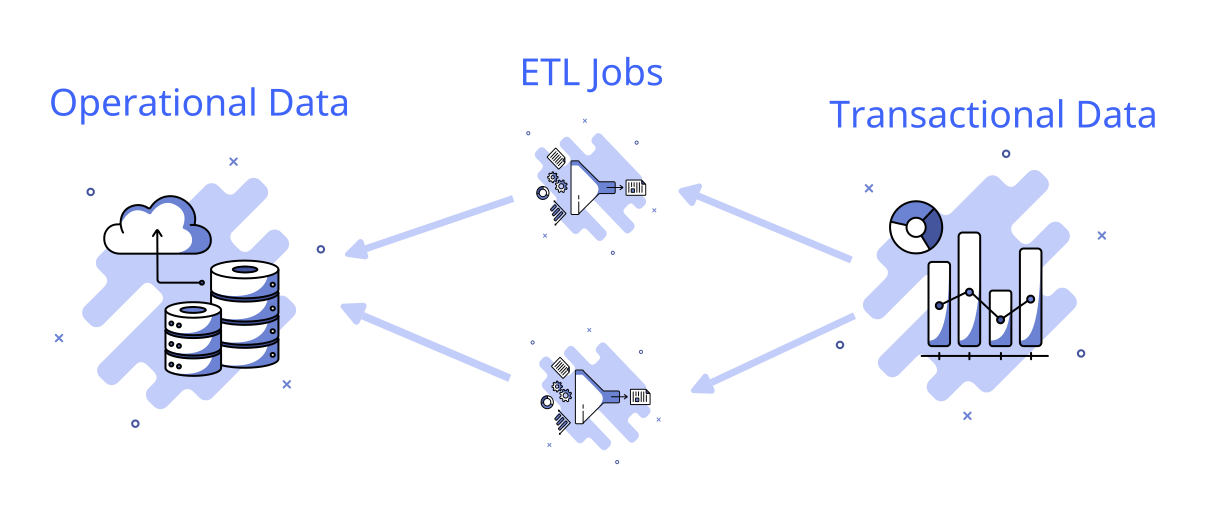
\includegraphics[width=\textwidth]{images/data-planes.png}
  \caption{The great divide of data}
  \label{fig:dataPlanes}
\end{figure}

Many of the technologies created over the years are developed underlying this very assumption. While these technologies are effective in handling the volume, velocity and variety of data, today's data challenges are about the proliferation of origins, data quality and data architecture. 

% For instance, intelligent pet healthcare would require longitudinal records on animal diagnostics, breed, environmental factors, particularities of the species, and even some of the owner's data. 

Data are usually collected and consolidated through several systems. Some of these data may even go beyond the perimeters of the organisation. Herefore, based on the premises discussed hereinabove and the challenges explicated in Section \ref{firstSLR:findings:limitationsOfCurrentRAs}, it is posited that today's data architectures need a shift from the centralization of data in one big analytical database to connecting analytical data wherever it is. 

Based on this, the artifact designed for this study learns from past solutions and addresses their shortcomings. This artifact aims to walk away from overly centralised and inflexible data architectures that act as a coordination bottleneck. Therefore, one of the objectives of this artifact is to bridge the gap between the point where data is generated and the point in which it is used, thus simplifying the process. This artifact aims to increase agility in the face of growth and respond effectively to organisational changes. Therefore the first architectural style of Metamycelium is as follows: 


\subsubsection{Localized autonomy through domain-driven decentralisation}

Today's businesses are dealing with a great deal of complexity. A typical business is made up of various domains with different domains and structures. These domains change at different rates and tend to be quite isolated from each other. The overall synergy of the business is dictated by the relationship between these domains and the ways in which these domains evolve. 

At the heart of these synergies sits volatility and rapid change in the market and an ever-increasing number of regulations. How do businesses today manage the impact of these changes to their data? should they constantly modify ETL jobs, create new ETL backlogs, and consolidate data into operational stores? how can businesses create quality and trustworthy data without slowing down? this boils down to embracing the change in today's data landscape. 

One way to tackle this complexity is to align technology with business. Businesses break down their problem into smaller problems that are handled in each domain; technology and data can be incorporated into those domains too. This approach is well-established in microservices architectures \cite{ataei2023application}. 

\subsubsection{Domain-driven design}


Integral to Metamycelium is the distribution and decentralisation of services into domains that have a clear, bounded context. Perhaps one of the most challenging things one might face when it comes to architecting a distributed system is: based on what architectural quanta should the system be broken down? This issue has been repeatedly discussed, for example, among adopters of microservices architecture \cite{DataMesh}. Metamycelium, inspired by the concept of domain-drive design (DDD), tends to sit data close to the product domain that relates to it. This implies that data is in the product domain and as a facet of it \cite{laigner2021data}.

This is mainly driven by the fact that most organisations today are decomposed based on their products. These products are the capabilities of the business that are segregated into various domains. These domains usually define their bounded context, evolve at different rates, and are operated by cross-functional teams \cite{teamtopologiesSkelton}. Incorporating data into these bounded contexts can result in a synergy that can improve the management of continuous change.

This can be micro, such as application developers communicating with data engineers about collecting user data in nested data structures, or macro, such as application developers thinking about redesigning their Graphql schema in an intermediary layer that may affect downstream analytical services. Therefore, the concept of DDD is incorporated into this study to facilitate communication and increase the adoption, rigour, and relevance of Metamycelium.

DDD is an approach to software development that focuses on understanding and modelling the problem domain of a software application. The goal of DDD is to create software that reflects the language, concepts, and behaviours of the problem domain rather than being based solely on technical considerations. 

DDD can help Metamycelium by providing a systematic approach to modelling and managing data that is closely aligned with the problem domain of the application. By focusing on the language, concepts, and behaviours of the problem domain, DDD can help data architects gain a deeper understanding of the data that is needed and how it should be structured (eridaputra 2014 modelling, DataMesh Communication is a key component of any software development endeavour \cite{sudhakar2012model}, and without it, essential knowledge sharing can be compromised. Often, data engineers and business stakeholders have no direct interaction with one another. Instead, domain knowledge is translated through intermediaries such as business analysts or project managers to a series of tasks to be done \cite{khrononov2021learning}. This implies at least two translations from two different ontologies.

In each translation, information is lost, which is essential domain knowledge, and this implies a risk to the overall quality of the data. In such a data engineering process, the requirement often gets distorted, and the data engineer has no awareness of the actual business domain or the problem being addressed.

Often, problems being solved through data engineering are not simple mathematical problems or riddles but rather have broader scopes. An organisation may decide to optimise workflows and processes through continuous data-driven decision-making, and a data architecture that is overly centralised and not flexible can risk project failure.


\subsubsection{Complex adaptive systems}

Architectures like Metamycelium share properties with complex adaptive systems \cite{holland1992complex}. The artifact designed for this thesis is especially inspired by the idea that powerful groups can emerge from an array of simple rules governing local agents. In one study, \citeauthor{reynolds1987flocks} analysed a synchronized flock of starling birds in autumn. This study presented the fact that every starling bird follows three simple rules: 1) alignment (following flockmates that are close by), 2) separation (so birds don't collide with each other), and 3) cohesion (keeping the same pace as the neighbouring flockmates). These rules can be mathematically expressed as follows:

Alignment:
$$
v_i(t+1) = v_i(t) + \frac{1}{k} \sum_{j=1}^{N} (v_j(t) - v_i(t))
$$

where $v_i(t)$ is the velocity vector of bird $i$ at time $t$, $k$ is a normalization factor, and $N$ is the number of neighbouring birds.

Cohesion:
$$
v_i(t+1) = v_i(t) + \frac{1}{k} (c_i(t) - p_i(t))
$$

where $c_i(t)$ is the center of mass of the neighbouring birds, $p_i(t)$ is the position of bird $i$ at time $t$, and $k$ is a normalization factor.

Separation:
$$
v_i(t+1) = v_i(t) + \sum_{j=1}^{N} \frac{(p_i(t) - p_j(t))}{d_{ij}^2}
$$

where $p_i(t)$ is the position of bird $i$ at time $t$, $p_j(t)$ is the position of bird $j$ at time $t$, and $d_{ij}$ is the distance between birds $i$ and $j$.

Starling birds don't need a centralised orchestrator to create this complex adaptive system. In Metamycelium the aim is to promote a domain-driven distribution of data ownership. This architecture is modeled in a way that a domain does not provide only operational data through a standard interface, but does provide analytical data too. For instance, in practice management software for veterinaries, the animal domain provides operational APIs for updating animal attributes, but it can also provide analytical interfaces for retrieving animal data within a window of time. Every domain owns its data.

In this fashion, the domain can also choose to retrieve data from other domains with some sort of discovery mechanism, process the data and enrich its data. In some cases, there can be a creation of aggregate domains with the main concern of aggregating data from various domains and providing it for a specific use case. 

This is to remove vertical dependency and allow teams to have their local autonomy while being empowered with the right level of discovery and APIs. This architecture promotes the idea of coequal nodes consolidated to achieve the overall goal of the system rather than a centralised database of all data owned by people who don't have domain knowledge. This concept is inspired by DDD in the book presented by \citeauthor{evans2004domain}, data mesh \cite{dehghani2020datamesh}, and microservices architecture \cite{newman2015building}.

\subsubsection{Event driven services}

Metamycelium's decentralized and distributed architecture introduces challenges in service communication as the network grows. Initially, simple point-to-point communication via REST API calls suffices, but this method proves inefficient with system expansion. Such synchronous interactions can lead to a 'distribution tax,' where one service's blocking state, often due to intensive processes, causes delays in dependent services \cite{montesi2016circuit}.

The heavy network demands of distributed systems may further complicate matters, potentially causing \emph{tail latency}, \emph{context switching}, and \emph{gridlocks} \cite{sriraman2018mu,gan2019open,kakivaya2018service,AtaeiApsec}. This tight coupling is at odds with the distributed system's goals of autonomy and resilience.

To overcome these issues, Metamycelium adopts asynchronous event-driven communication. This model enables services to publish and respond to events, thus decoupling their interactions. In this \emph{publish and forget} framework, services announce events to specific topics and move forward without awaiting direct responses. This is similar to restaurant staff responding to environmental cues instead of direct commands, promoting a smooth operational flow.

While event-driven architectures typically offer eventual consistency, which might not be suitable for certain real-time stream processing scenarios requiring immediate consistency, it is a safe assumption that the majority of data engineering workloads can efficiently operate within an event-driven paradigm.

According to \citeauthor{richards2020fundamentals}, event-driven architectures come in two major topologies: 1) broker topology and 2) mediator topology. Additionally, in the works of \citeauthor{stopford2018designing} the concept of streaming platforms is elaborated. Since Metamycelium is a BD architecture that aims to process analytical data, a lot of challenges of achieving ACID transactions are eliminated. Therefore Metamycelium adopts the architectural concepts of \emph{distributed asynchronous event-driven systems} using a hybrid topology. That is, Metamycelium is absorbing some elements of the broker topology, some elements of the mediator topology and many concepts from streaming platforms. Therefore in Metamycelium's CAP theorem \cite{brewer2000towards} partition tolerance and availability are top guarantees. 

There are five primary architectural components within this hybrid topology: the event, the event consumer, the event producer, the event backbone and the eventing interface. Events are initiated by the event producer and are dispatched to the topic of interest. This event then goes through the event broker and is stored there for retrieval in a queue-like indexed data structure. The event consumers that are interested in this topic will then listen to the topic of interest using the eventing interface. The event backbone itself is internally a distributed system that is made up of an arbitrary number of event brokers. 

Event brokers are services that are spawned and provisioned to facilitate event communication through Metamycelia. These brokers are coordinated with a distributed service coordinator. Brokers do also allow for the replication of topics. Furthermore, to allow for fault tolerance and recoverability, the event backbone has a dedicated event archive. This archive aims to store all events that are going through the brokers so they can be restored to a correct state if a failure occurs. 


% Moreover, all events that are getting sent into the event backbone through the producer and all events that are being received from the even consumer go through schema validation. Schemas are defined and checked against all events from the domain in order to avoid hard-to-find issues and service failure. These schemas are part of the metadata API discussed in Section~\ref{section:aNewArchitecturalQuantum:metadata}.

These components work together to create a distributed, fault-tolerant, and scalable data system that can handle both batch and stream processing as portrayed in Figure \ref{fig:eventDrivenArchitecture}. 

\begin{figure}[h]
  \centering
  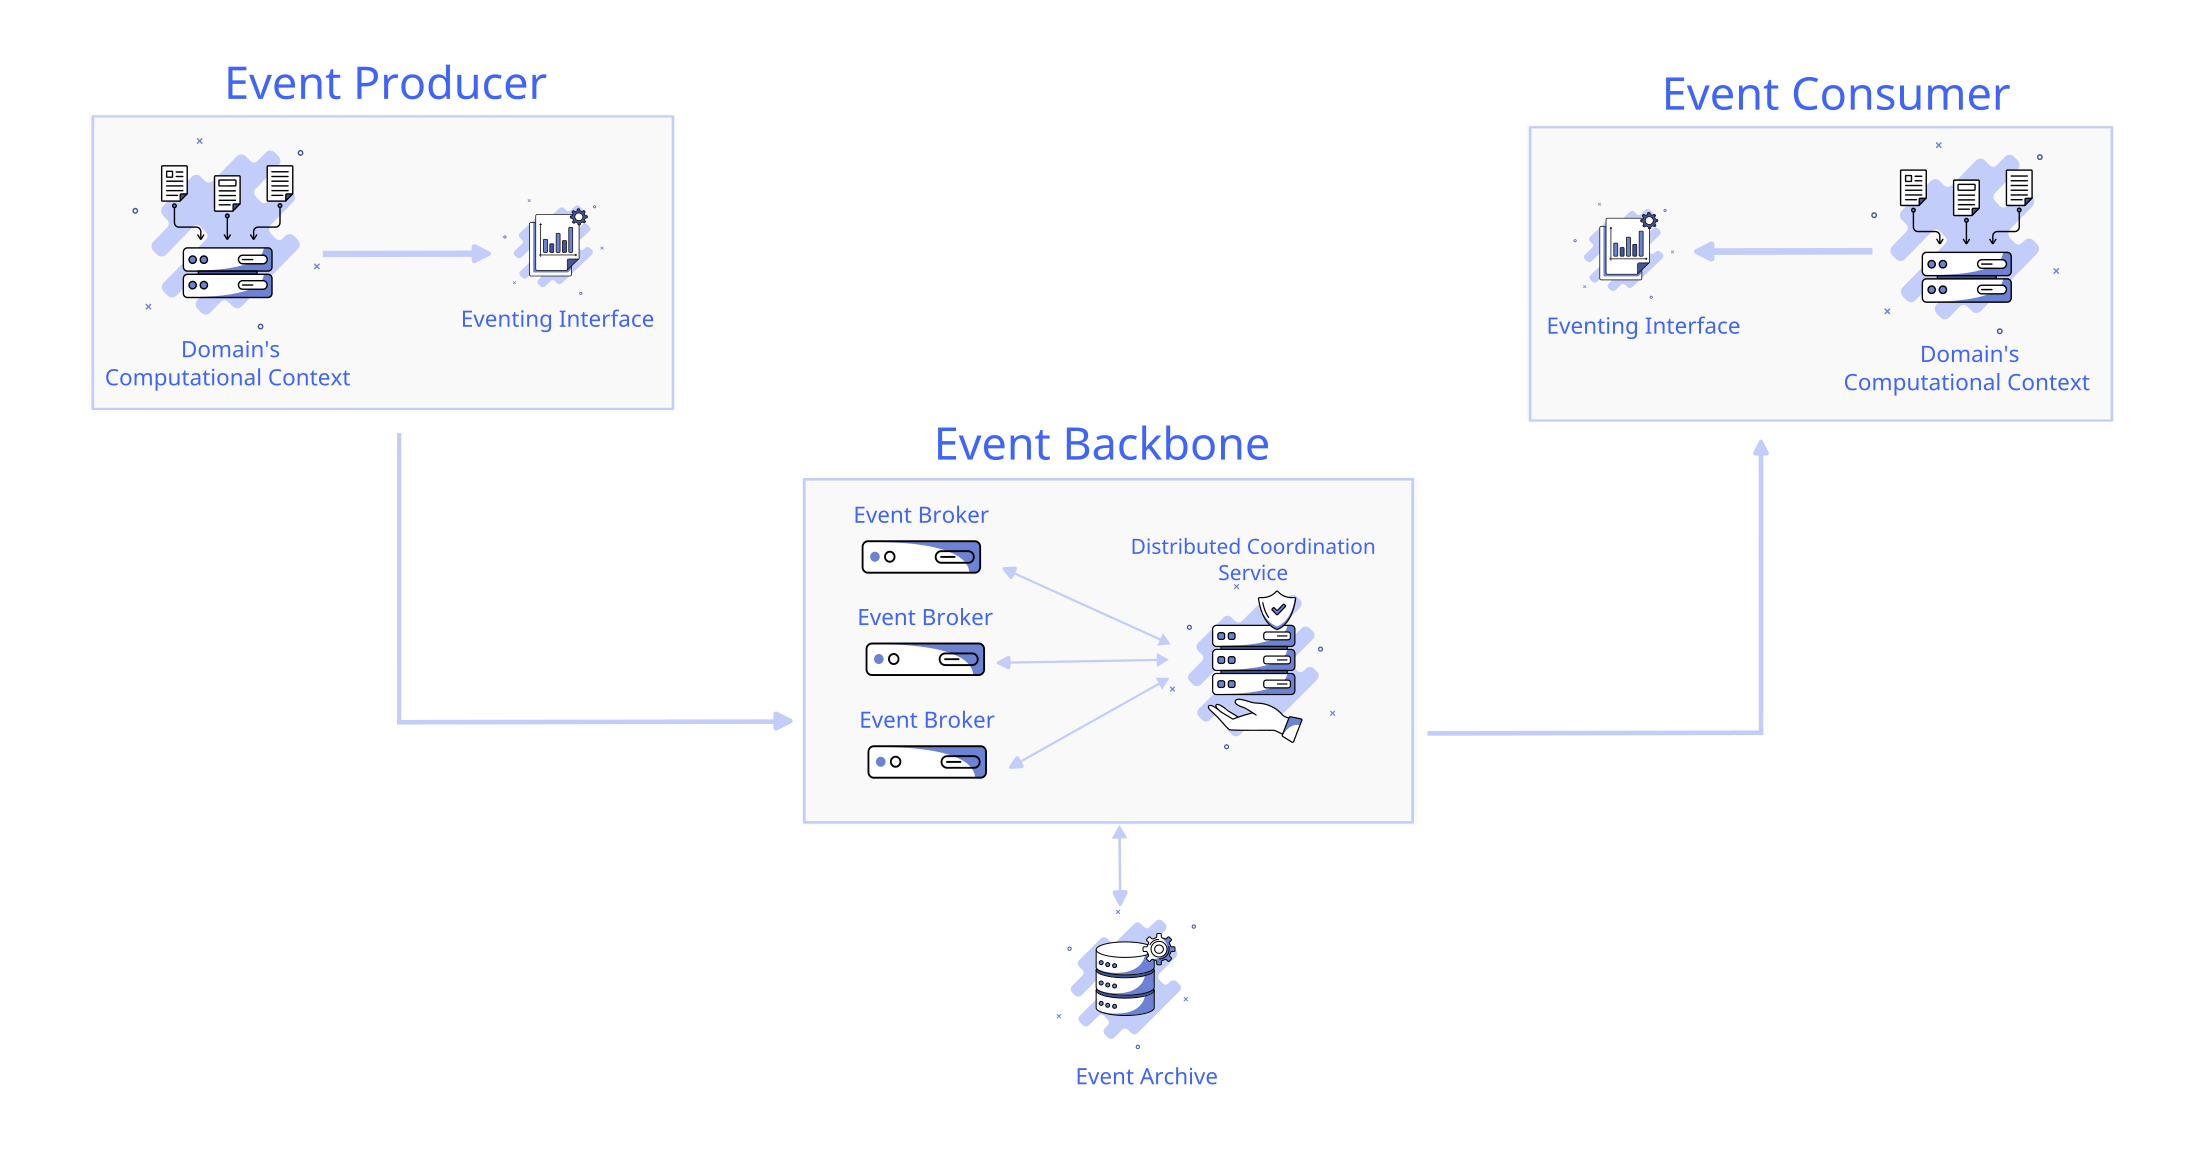
\includegraphics[width=\textwidth]{images/Event-architecture.png}
  \caption{Metamycelium Event-driven Architecture}
  \label{fig:eventDrivenArchitecture}
\end{figure}


\subsection{Architectural characteristics}

The architectural characteristics of the Metamycelium architecture are notable for their focus on maintainability, scalability, fault tolerance, elasticity, and deployability. It aligns with modern engineering practices such as automated deployment and continous integration. The architecture emphasises the use of microservices, which are independently deployable and maintainable components.

Maintainability is a high-scoring characteristic of this architecture. The use of event-driven microservices architecture allows for modular development and independent scaling, making it easier to maintain and update individual components without affecting the entire system. Additionally, the architecture supports automated deployment practices, facilitating efficient updates and reducing manual intervention.

Scalability and elasticity are also prominent features. The architecture enables horizontal scalability, allowing for the addition or removal of services based on demand. This flexibility ensures that the system can handle varying workloads effectively.

Fault tolerance is another strength of the architecture. While interservice communication can impact fault tolerance, redundant and scalable design of Metamycelium, along with service discovery mechanisms, mitigate this issue. The independent, single-purpose nature of microservices generally leads to high fault tolerance.

Deployability is emphasised, thanks to the small deployment units and decoupled nature of Metamycelia. The architecture supports evolutionary change, aligning with modern business practices that require agility and adaptability. Small, independently deployable units allow for faster updates and iterations, keeping pace with the dynamic nature of business requirements.

However, the architecture may receive a lower score in terms of cost and simplicity. The distributed nature of Metamycelium and the potential for increased communication overhead can introduce complexities in managing and optimizing costs. Strategies such as intelligent data caching and replication can address performance challenges associated with network calls, but cost management remains an ongoing consideration.

Overall, the Metamycelium architecture embraces the strengths of microservices, prioritising maintainability, scalability, fault tolerance, elasticity, and deployability. It acknowledges the challenges inherent in distributed architectures and offers strategies to mitigate them. Architects must understand the rules of architecture to intelligently navigate and leverage its benefits effectively. An overview of architectural characteristics is portrayed in Table~\ref{tab:architecture-characteristics}

\begin{table}
  \centering
  \caption{Metamycelium Architecture Characteristics}
  \label{tab:architecture-characteristics}
  \begin{tabular}{|l|c|}
    \hline
    \textbf{Characteristic} & \textbf{Score} \\
    \hline
    Maintainability & $\bigstar\bigstar\bigstar$ \\
    \hline
    Scalability & $\bigstar\bigstar\bigstar\bigstar$ \\
    \hline
    Fault Tolerance & $\bigstar\bigstar\bigstar$ \\
    \hline
    Elasticity & $\bigstar\bigstar\bigstar\bigstar$ \\
    \hline
    Deployability & $\bigstar\bigstar\bigstar\bigstar$ \\
    \hline
    Cost & $\bigstar\bigstar$ \\
    \hline
    Simplicity & $\bigstar$ \\
    \hline
    Performance & $\bigstar\bigstar\bigstar$ \\
    \hline
    Support for Modern Engineering Practices & $\bigstar\bigstar\bigstar\bigstar$ \\
    \hline
  \end{tabular}
\end{table}

\section{Artifact}
\label{sec:artifact}
% Describe the design and development of the reference architecture artifact, focusing on its structure and components.

\section{Discussion}
\label{sec:discussion}
% Reflect on the findings from the evaluation, discussing their implications, limitations, and the relevance to existing and future research.

\section{Conclusion}
\label{sec:conclusion}
% Summarize the main contributions of your paper, its practical implications, and suggest directions for future research.




\appendix




\bibliographystyle{elsarticle-harv}
\bibliography{bibfile}

\end{document}
\endinput
%%
%% End of file `elsarticle-template-num.tex'.